\documentclass[12pt,]{article}
\usepackage[left=1in,top=1in,right=1in,bottom=1in]{geometry}
\newcommand*{\authorfont}{\fontfamily{phv}\selectfont}
\usepackage{lmodern}


  \usepackage[T1]{fontenc}
  \usepackage[utf8]{inputenc}



\usepackage{abstract}
\renewcommand{\abstractname}{}    % clear the title
\renewcommand{\absnamepos}{empty} % originally center

\renewenvironment{abstract}
 {{%
    \setlength{\leftmargin}{0mm}
    \setlength{\rightmargin}{\leftmargin}%
  }%
  \relax}
 {\endlist}

\makeatletter
\def\@maketitle{%
  \newpage
%  \null
%  \vskip 2em%
%  \begin{center}%
  \let \footnote \thanks
    {\fontsize{18}{20}\selectfont\raggedright  \setlength{\parindent}{0pt} \@title \par}%
}
%\fi
\makeatother




\setcounter{secnumdepth}{0}


\usepackage{graphicx}
% We will generate all images so they have a width \maxwidth. This means
% that they will get their normal width if they fit onto the page, but
% are scaled down if they would overflow the margins.
\makeatletter
\def\maxwidth{\ifdim\Gin@nat@width>\linewidth\linewidth
\else\Gin@nat@width\fi}
\makeatother
\let\Oldincludegraphics\includegraphics
\renewcommand{\includegraphics}[1]{\Oldincludegraphics[width=\maxwidth]{#1}}

\title{A conceptual typology for the population impacts of sea level rise \thanks{All data and code that supports these conclusions are available as
supplementary materials.}  }



\author{\Large Mathew E. Hauer*\vspace{0.05in} \newline\normalsize\emph{Florida State University}   \and \Large R. Dean Hardy\vspace{0.05in} \newline\normalsize\emph{University of Maryland}   \and \Large Scott Kulp\vspace{0.05in} \newline\normalsize\emph{Climate Central}   \and \Large Robert Kopp\vspace{0.05in} \newline\normalsize\emph{Rutgers University}   \and \Large Michael Oppenheimer\vspace{0.05in} \newline\normalsize\emph{Princeton University}  }


\date{}

\usepackage{titlesec}

\titleformat*{\section}{\normalsize\bfseries}
\titleformat*{\subsection}{\normalsize\itshape}
\titleformat*{\subsubsection}{\normalsize\itshape}
\titleformat*{\paragraph}{\normalsize\itshape}
\titleformat*{\subparagraph}{\normalsize\itshape}


\usepackage{natbib}
\bibliographystyle{apsr}
\usepackage[strings]{underscore} % protect underscores in most circumstances



\newtheorem{hypothesis}{Hypothesis}
\usepackage{setspace}

\makeatletter
\@ifpackageloaded{hyperref}{}{%
\ifxetex
  \PassOptionsToPackage{hyphens}{url}\usepackage[setpagesize=false, % page size defined by xetex
              unicode=false, % unicode breaks when used with xetex
              xetex]{hyperref}
\else
  \PassOptionsToPackage{hyphens}{url}\usepackage[unicode=true]{hyperref}
\fi
}

\@ifpackageloaded{color}{
    \PassOptionsToPackage{usenames,dvipsnames}{color}
}{%
    \usepackage[usenames,dvipsnames]{color}
}
\makeatother
\hypersetup{breaklinks=true,
            bookmarks=true,
            pdfauthor={Mathew E. Hauer* (Florida State University) and R. Dean Hardy (University of Maryland) and Scott Kulp (Climate Central) and Robert Kopp (Rutgers University) and Michael Oppenheimer (Princeton University)},
             pdfkeywords = {},  
            pdftitle={A conceptual typology for the population impacts of sea level rise},
            colorlinks=true,
            citecolor=blue,
            urlcolor=blue,
            linkcolor=magenta,
            pdfborder={0 0 0}}
\urlstyle{same}  % don't use monospace font for urls

\usepackage[all]{nowidow}
\usepackage{rotating}
\usepackage{fancyhdr}
\usepackage[table]{xcolor}
\usepackage{tabularx}
\usepackage{makecell}
\usepackage{xcolor}
\pagestyle{fancy}
\fancyhead{}
\fancyhead[CE,CO]{SLR typology}


% add tightlist ----------
\providecommand{\tightlist}{%
\setlength{\itemsep}{0pt}\setlength{\parskip}{0pt}}

\begin{document}
	
% \pagenumbering{arabic}% resets `page` counter to 1 
%
% \maketitle

{% \usefont{T1}{pnc}{m}{n}
\setlength{\parindent}{0pt}
\thispagestyle{plain}
{\fontsize{18}{20}\selectfont\raggedright 
\maketitle  % title \par  

}

{
   \vskip 13.5pt\relax \normalsize\fontsize{11}{12} 
\textbf{\authorfont Mathew E. Hauer*} \hskip 15pt \emph{\small Florida State University}   \par \textbf{\authorfont R. Dean Hardy} \hskip 15pt \emph{\small University of Maryland}   \par \textbf{\authorfont Scott Kulp} \hskip 15pt \emph{\small Climate Central}   \par \textbf{\authorfont Robert Kopp} \hskip 15pt \emph{\small Rutgers University}   \par \textbf{\authorfont Michael Oppenheimer} \hskip 15pt \emph{\small Princeton University}   

}

}








\begin{abstract}

    \hbox{\vrule height .2pt width 39.14pc}

    \vskip 8.5pt % \small 

\noindent This paper provides a conceptual framework for assessments of the
impacts of sea level rise on populations. Population impact assessments
of sea level rise are common in the literature and such assessments
directly influence our understanding of the societal effects of climate
change and sea level rise. However, these assessments typically limit
population exposure to inundation areas only. Drawing on increasingly
sophisticated flood modeling, we propose a new typology for
understanding population exposure risk to sea level rise based on a
spatial envelope probability of exposure to tidal flooding approach. The
typology identifies three types of exposure risk: direct, indirect, and
tertiary. Implications and effects of sea level rise on each exposure
risk typology is then discussed. Using Chatham County, Georgia as an
example, we find that current assessments could grossly underestimate
both the spatial and temporal dimensions of the societal impacts of sea
level rise. The typology can be used to guide new research, assist with
impact assessments, evaluate policy options, and provide more robust and
holistic scenarios of sea level rise.


    \hbox{\vrule height .2pt width 39.14pc}


\end{abstract}


\vskip 6.5pt


\noindent \doublespacing *Corresponding author.
\href{mailto:mehauer@fsu.edu}{\nolinkurl{mehauer@fsu.edu}} p:
850-542-9369.

\hypertarget{introduction}{%
\section{Introduction}\label{introduction}}

The societal impacts of climate change and sea level rise (SLR) are of
utmost importance in the 21st century and climate assessments are an
integral part of adaptation and risk management
\citep{howden2016innovations}. Research has long sought to identify the
impact of sea level rise on society
\citep{curtis2011understanding, wu2002vulnerability}, with an increasing
focus on estimation of at-risk populations associated with sea level
rise \citep{curtis2011understanding, strauss2015carbon}. With 40\% of
the US population living in a NOAA designated coastal community
\citep{ache2015coast} and over one billion people living in coastal
areas around the world \citep{neumann2015future}, questions on the
societal impacts of sea level rise continue to be asked.

One of the primary components of a climate assessments of the impacts of
sea level rise involves calculating at-risk populations. A wide variety
of definitions of `at-risk' populations have been utilized including the
populations in lower-elevation coastal zones
\citep{neumann2015future, mcgranahan2007rising}, populations under the
mean higher high water (MHHW) mark
\citep{hauer2016millions, strauss2015carbon}, and populations in the
100-year flood plain
\citep{nicholls2010sea, brown2018quantifying, hallegatte2011assessing, heberger2011potential}.
All three approaches conceptualize at-risk populations as binary
outcomes, ie populations are either at-risk or not at-risk, located
within specific geographies defined through each approaches'
characterization schema and share shortcomings related to an equality of
risk, an equality of temporal exposure, and an equality of exposure.
First, these approaches presume an equality of risk within each
geography assuming a homogenous risk profile across heterogeneous
terrain. For instance, in a flood plain based approach, all populations
in the 100-year flood plain are implicitly assumed to have equal flood
risk, despite certain populations living in the 10-year or 20-year flood
plain. Second, these approaches presume an equality of temporal
exposure. For populations living within 0.9m of the current MHHW mark,
those living within 0.1-0.2m of the MHHW mark will surely experience
effects of sea level rise sooner than those living in the 0.8-0.9m mark.
And lastly, these approaches presume an equality of exposure. For
populations living in a lower-elevation coastal zone, some will be
exposed to sea level rise and others won't be exposed to sea level rise
but could be exposed to other associated hazards such as storm surges
and other livelihood impacts. These shortcomings combine to create a
gross oversimplification of the extent, timing, exposure, and ultimately
adaptation options for coastal communities.

In this paper, we compare and contrast these three theoretical, binary
approaches and suggest a unified typology for investigating exposure to
sea level rise using a probability spatial envelope typology. We
characterize exposed populations into three main categories: directly
impacted, indirectly impacted, and tertiary impacted. These categories
combine the strengths of all three previous approaches into a single
unified framework. We then examine the implications for this novel
framework within the context of Chatham County, Georgia.

\hypertarget{conceptual-models-in-the-literature}{%
\section{Conceptual Models in the
Literature}\label{conceptual-models-in-the-literature}}

The way populations exposed or at-risk to sea level rise are
conceptualized drives the societal impacts from SLR. Assessments using
lower-elevation coastal zones, for instance, use generalized risk
allocations that can frame climate adaptation discussions across the
widest possible area. It is not just simply SLR, but rather a
combination of SLR, recurrent tidal flooding, and elevated risk of
disastrous storm surges that comprise the full range of effects
associated with sea level rise. However, more explicit spatiotemporal
linkages to localized SLR hazards is clearly warranted. Adaptation
strategies for those currently living under 1.8m of elevation, the
``high'' scenario of sea level rise expected in the 21st century
\citep{sweet2017global}, are inherently different from those living
above 1.8m of elevation but still within the LECZ. Appropriate
accounting of type of exposure to the hazards of sea level rise would
improve upon our current frameworks.

Recent tidal events in the Atlantic Coast of the United States and
elsewhere
\citep{carbognin2010global, spanger2014encroaching, dahl2017sea} have
demonstrated that the impacts of rising sea levels are advancing further
and faster than those indicated by inundation models that assess impacts
at mean higher high water (MHHW). The increased frequency and magnitude
of tidal flooding in coastal communities can be considered as the
immediate impact of sea level rise (SLR). Perigean spring tide events
cause regularly recurring water levels well above MHHW, and in many
parts of the coast this causes significant flooding, sometimes referred
to as nuisance flooding or recurring tidal flooding
\citep{fennessey2001changes}, particularly when these tidal events are
supported by significant onshore winds from tropical cyclones or storms.
Mean higher high water does not mark the highest extent of regularly
occurring tide waters as the tide range will naturally exceed this level
approximately half of the time, as its name suggests. Assessments using
impacts from changes in MHHW inadvertently turn a blind eye to the
potential impacts of sea level rise on areas above the MHHW mark.
However, property just above the MMHW mark will be regularly flooded
long before it transitions below the MHHW mark, thus individuals and
properties would not be counted as impacted, despite being regularly
flooded by tides that exceed MHHW with added SLR. This is especially
important in areas with large variations in their tidal datums.

A more broad approach involves utilizing either lower-elevation coastal
zones or the 100-year flood plain to characterize the populations
exposed to hazards from sea level rise
\citep{hallegatte2011assessing, neumann2015future}. In this way,
populations within these geographies are framed as having equal risk
regardless of their location within the LECZ or the 100-year flood
plain. This approach has a side effect of equalizing the temporal
horizon of hazards associated with sea level rise. By characterizing all
populations in the LECZ or the 100-year flood plain as being at-risk to
the hazards associated with sea level rise, regardless of either the
extent of sea level rise or the timing of the rise. In other words, both
lower elevation coastal zones and 100-year flood plain approaches render
any coastal population as exposed to sea level rise in any time period.
This has an unintended consequence of inflating sea level rise hazards
as all coastal populations are effectively ``exposed'' to sea level rise
and makes it difficult to decompose the effect of sea level rise on
typical coastal hazards. Shoreline populations in areas with tropical
cyclone activity are already exposed to storm surges, for instance,
regardless of sea level rise. Which additional populations will be
exposed to storm surges due to a higher base water level becomes
increasingly difficult with a LECZ or 100-year flood plain approach.

\begin{figure}
\centering
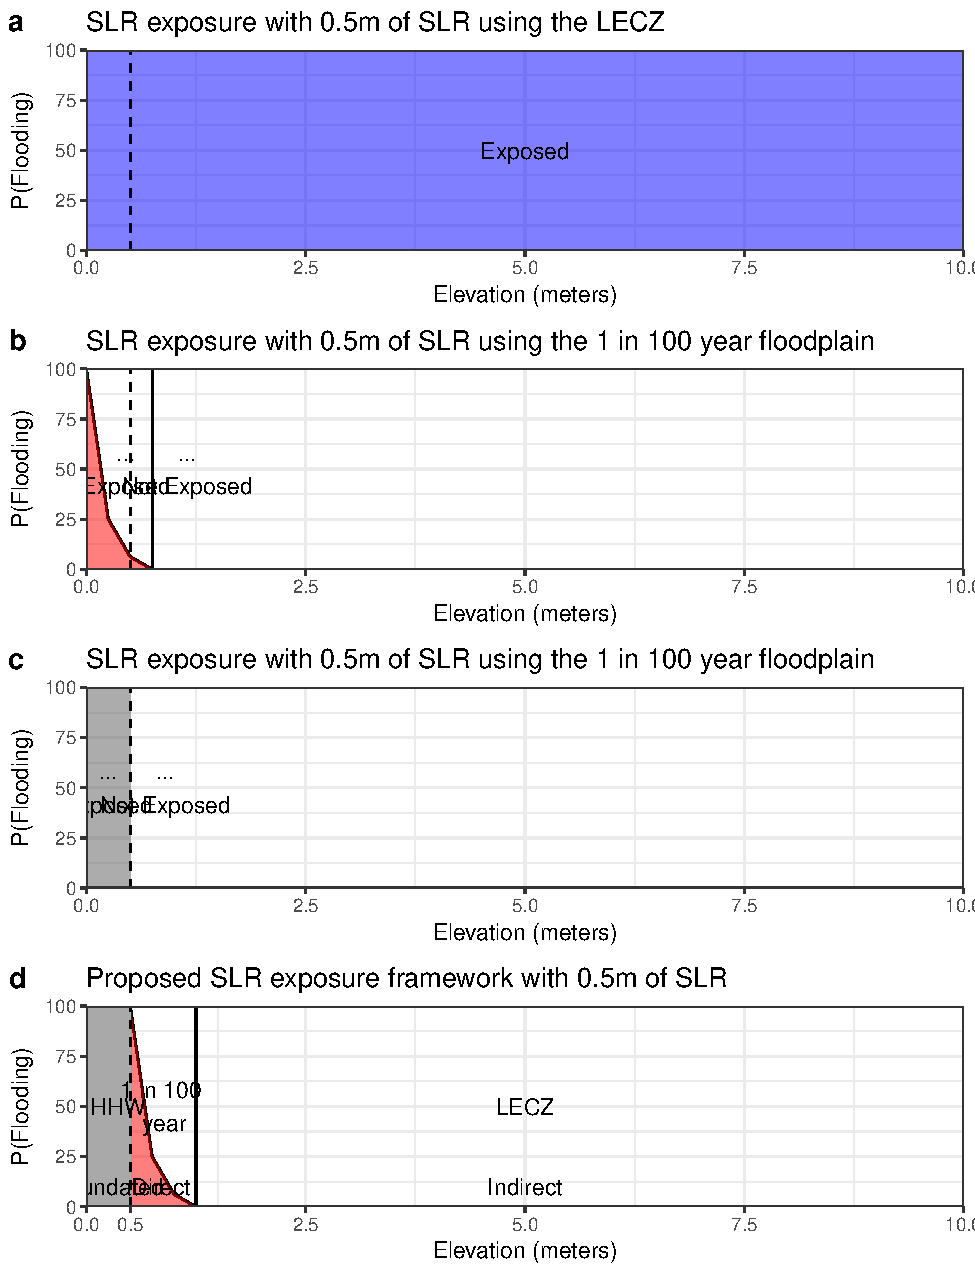
\includegraphics{SLR_typology_files/figure-latex/pastexamples-1.pdf}
\caption{\textbf{SLR typology outline.} The vertical dashed line
represents 0.5m of SLR, the solid vertical line represents the exposed
population using a floodplain approach. \label{figure1}}
\end{figure}

\autoref{figure1} summarize the current conceptual models for examining
the impacts of sea level rise. Panels a, b, and c in Figure 1
demonstrate conceptually who is at risk of SLR assuming 0.5m of SLR.
Using a LECZ conceptualization (a), all persons within the LECZ are
assumed to be exposed to SLR. Using the 1 in 100 year floodplain
conceptualization (b), all persons below a given elevation are assumed
to be at risk despite reduced flood risks at higher elevations. Using a
MHHW conceptualization (c), only those persons who have exactly 100\%
probability of flooding are considered at risk.

\hypertarget{a-unified-conceptual-model}{%
\section{A Unified Conceptual Model}\label{a-unified-conceptual-model}}

When taken together, these three models capture all possible hazards
associated with sea level rise but are plagued by issues on an
individual conceptual basis. We propose a new model, unifying the MHHW,
LECZ, and 100-year floodplain approaches into a more conceptually sound
framework based on a spatial envelope, probability of exposure model. In
a departure from the other three models' characterizations of at-risk
and not at-risk, we characterize exposure to sea level rise as
\textbf{inundated}, \textbf{direct}, and \textbf{indirect} based on a
location's probability of flooding within spatial envelopes. A three
tiered exposure approach allows for a pliable examination of both hazard
exposure and adaptive options.

We characterize those who are \textbf{inundated} as those people living
below the future MHHW mark. These are the populations who will be the
most adversely affected, will experience impacts from sea level rise the
soonest, and who are directly threatened by inundation if adaptive
measures are not undertaken. Inundation exposure is analogous to the
population's risk understood through the MHHW approach discussed above.
Eventually, these populations will experience water levels above their
elevation 50\%+ of the time. These areas are typically discussed in
conversations concerning managed retreats
\citep{huntington2012towards, hino2017managed}. Such areas will be
directly affected as soon as 2045 under some of the most aggressive sea
level rise curves
\citetext{\citealp{deconto2016contribution}; \citealp[@][]{sweet2017global}}.

We characterize those who are \textbf{directly} exposed to sea level
rise as those people who are living above the future MHHW mark, but
below the spatial extent of future flooding from sea level extremes or
tidal flooding. These are the populations exposed to recurrent or
nuisance flooding \citep{chang2010potential, dahl2017sea} and will
experience water levels above their elevation less than 50\% of the
time. These areas are typically not discussed in the context of managed
retreats, but are frequently discussed regarding adaptive measures such
as elevating roads \citep{titus2009state}, coastal armoring
\citep{jin2015shoreline}, or other near-term adaptations.

Finally, we characterize those who are \textbf{indirectly} exposed to
sea level rise as living in areas above both the MMHW mark and the
extent of future tidal flooding, but in neighborhoods that are directly
or semi-directly at risk to sea level rise. Here, we conceptualize the
rest of the areas located in a LECZ or 100-year floodplain or other
coastal geography. While these areas are not likely to see their
properties exposed to elevated sea levels, the people in these areas
will likely drive on flooded roads, go to workplaces in flooded areas,
and could see their property values depressed \citep{neumann2015joint}.

Our frameowkr bases SLR exposure on both flood exposure, expressed here
as probability of flooding, and geographic location. We can also see the
presence of indirectly impacted populations under current conditions
(\textbackslash{}autoref\{figure1). Sea level rise is typically imagined
as a hazard typified by long range time horizons up to 2,000 years into
the future \citep{strauss2015carbon}, but related impacts from sea level
rise, specifically manifested as coastal flooding, are occurring today
in parts of the Atlantic Coast of the United States and Venice, Italy,
for instance.

To demonstrate the differences in impacts under our proposed model
compared to previous frameworks, we use an empirical example of Chatham
County, Georgia (\autoref{figure2}). Chatham County is an ideal platform
for demonstrating the various populations exposed to sea level rise in
our conceptual model. It is a coastal county with a Census 2010
population of approximately 266,000, making it a medium-sized area, and
it is typified by its coastal marsh ecosystem and very large
astronomical tides. It has also been identified as having approximately
10\% of its population at risk to sea level rise using a MHHW approach
\citep{hauer2016millions}.

We use the National Oceanographic and Atmospheric Administration's
(NOAA) sea level rise database that simulate expected changes in the
mean higher high water (MHHW) mark on areas that are hydrologically
connected to coastal areas for the 0ft through 5ft datasets. These
datasets does not take into account additional land loss caused by other
natural factors such as erosion, subsidence, or future construction and
NOAA provides these data ``as is'' without warranty to their
performance. Land lost due to sea level rise is calculated with a
spatial overlay workflow in ArcGIS 10.1 as one minus the percentage of
land lost under the 0ft base layer of sea level rise, ie 1ft divided by
0ft, 2ft divided by 0ft, etc. The first step in the analysis was to
utilize a base, 0ft Mean Higher High Water (MHHW) layer, which was
derived from NOAA's 0ft scenario, and used as the initial condition to
calculate a base of dry land area contained within the geographies of
2010 Census Block Groups. The resulting calculation is therefore a total
area of dry land currently available for human habitation within each
Census Block Group geography.

We used an area based approach \citep{hauer2016millions} to classify
populations as inundated, directly, or indirectly impacted using Census
Block Group geographies through the following sets of equations in Table
X. All populations reported come from Census 2010.

\begin{table}
\centering
\caption{My caption}
\label{my-label}
\begin{tabular}{|l|l|}
\hline
Inundated  & $PR_j^s=P_j \,\, \cdot \,\, \frac{A_j^s}{A_j^0}$ \\ \hline
Directly   & $PR_j^s=P_j \,\, \cdot \,\, \frac{A_j^{s+}}{A_j^0}$ \\ \hline
Indirectly & $\frac{A_j^{s+}}{A_j^0}>0,\,\, Indirectly=P_j$    \\ \hline
\end{tabular}
\end{table}

Where the population at risk of being impacted (\(PR_j^s\)) under
scenario \(s\) in census block group \(j\) is equal to the population
(\(P\)) in census block group \(j\) multiplied by the ratio of dry land
area (\(A_j^s\)) in census block group \(j\) under sea level rise
scenario \(s\) to the dry land area under 0ft of sea level rise
(\(A_j^0\)). For indirectly and tertiary impacted areas, we use \(s+\)
to denote the dry land area under sea level rise scenario \(s\) plus the
highest astronomical tide. For Chatham County, this is roughly
equivalent to approximately 2ft above the MHHW mark.

\begin{figure}
\centering
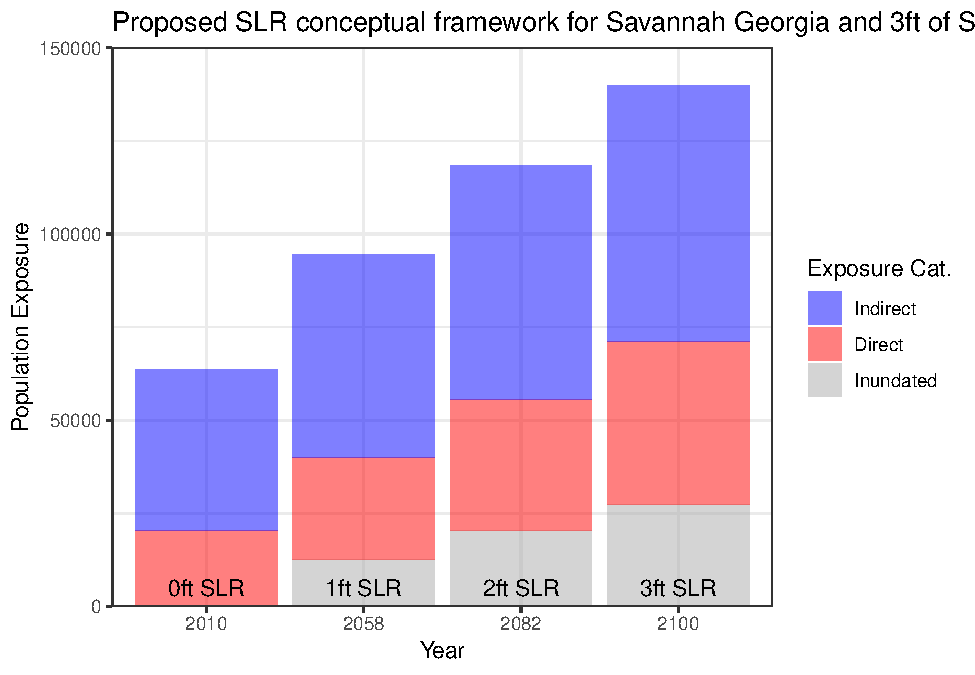
\includegraphics{SLR_typology_files/figure-latex/savannah-1.pdf}
\caption{\textbf{Proposed SLR typology effect in Chatham County, GA} The
vertical dashed line represents 0.5m of SLR, the solid vertical line
represents the exposed population using a floodplain approach.
\label{figure2}}
\end{figure}

\autoref{figure2} shows the results for all three at-risk
classifications under current conditions (0ft) through 3ft of SLR. We
can see that the narrowest interpretation of exposure to sea level rise
(\textbf{inundated}), roughly corresponds to those who will be inundated
by MHHW, represents the smallest exposed population. Approximately
12,000 people could be directly exposed with 1ft of SLR, growing to
approximately 27,000 with 3ft of SLR. Those who could be exposed to
coastal flooding, or \textbf{directly exposed}, currently sits at
approximately 21,000 people under a 0ft, baseline sea level rise
scenario representing current conditions. This nearly doubles to
approximately 43,000 people with 3ft of SLR. Lastly, we see that those
who live in neighborhoods that will experience flooding is currently
approximately 63,000 but grows to nearly 140,000 with just 3ft of SLR.

\hypertarget{relation-to-adaptation}{%
\subsection{Relation to Adaptation}\label{relation-to-adaptation}}
\newpage
\singlespacing 
\bibliography{LATEX/mybibfile}
\end{document}